% Homework 1
\documentclass[12pt, letterpaper]{article}

\usepackage[top=1in, bottom=1.5in, left=.5in, right=.5in]{geometry}
\usepackage[colorlinks=true,urlcolor=blue,citecolor=blue]{hyperref}
\usepackage{graphicx}
\usepackage{enumerate}
\usepackage{natbib}
\usepackage{amsmath}

% Force pdflatex to use correct paper size.
\special{papersize=8.5in,11in}
\setlength{\pdfpageheight}{\paperheight}
\setlength{\pdfpagewidth}{\paperwidth}

\begin{document}

\begin{center}
  {\LARGE \textbf{Computational Science Qual Question}}\\
\end{center}

After working with the forward-difference method program that we created
in class, you have found that the stability criteria is proving to be a
limiting factor in getting your projects done in a timely fashion.  If you
were able to take larger time steps, you could finish your simulations faster
and be more productive.  However, you cannot do so without the result
becoming unstable and meaningless.

Enter \emph{Ace Zerblonski}, 8$^{th}$ year grad student extraordinaire.  Upon
seeing your plight, he says that you should be using the 
\textbf{Crank-Nicholson} scheme, which is unconditionally stable and 
second-order accurate in both time and space.  Your forward-difference scheme
is only first order accurate in time.  With such a solver, you could obtain
accurate results with far fewer time steps!

Ace mentions that he has a Fortran module that can solve the heat equation
using this method, but it comes with some caveats.
\begin{itemize}
  \item It depends on LAPACK, a linear algebra package.  Ace says that this
    isn't a problem because LAPACK is on most computers already.
  \item It also depends on a module called \textit{ModWrite2d.f90}, but
    Ace doesn't have this file any more.  He says this shouldn't be a problem
    because you can just write your own.
  \item When you ask if the module works, Ace says, ``probably, but I didn't
    test it or anything, man.''  
\end{itemize}

You ask Ace for more help, but he mumbles something about going on vacation
and leaves the office.  
Beyond some comments in the code, you're on your own.
Realizing that you need results for an upcoming
conference, you decide that your best option is to use this untested 
module.  Ace is a decent programmer, so you suspect that the file works, but
you are not \emph{certain} that it works.  

One way to \emph{quantitatively} show that a solver works is to investigate
the error, i.e., the difference between a known solution and the numerical
solution.  You know that error $\propto \Delta x^n$, where $\Delta x$ is either
a time step or spatial step and n is the ``order'' of the solver.  
This means that if you halve the time step for an $n^{th}$ order scheme, the 
error should reduce by a factor $\frac{1}{2^n}$.  If you were to run your code 
for many different time or spatial steps and calculate the error, then plot
error-versus-step size on a log-log scale, you would expect Figure~\ref{f1} to
develop.  For extremely small $\Delta t$, floating point error is the main
contributor to the total, so the error stays flat.  At very large values of
$\Delta t$, the time step is not appropriate for the problem at hand, so the
error oscillates unpredictably.  In between, however, we enter the 
\emph{asymptotic regime}, where the slope of the curve reflects the 
order-of-accuracy (in time) of the selected solver.  Such a result
quantitatively verifies that the solver tested in Figure \ref{f1} is 
implemented correctly \cite[e.g.,][]{Roache:1998}.  Note that it is possible
to apply this methodology even when no analytical solution exists
\cite[][]{Roache:2002}.

\begin{figure}[h]
  \vspace*{2mm}
  \begin{center}
    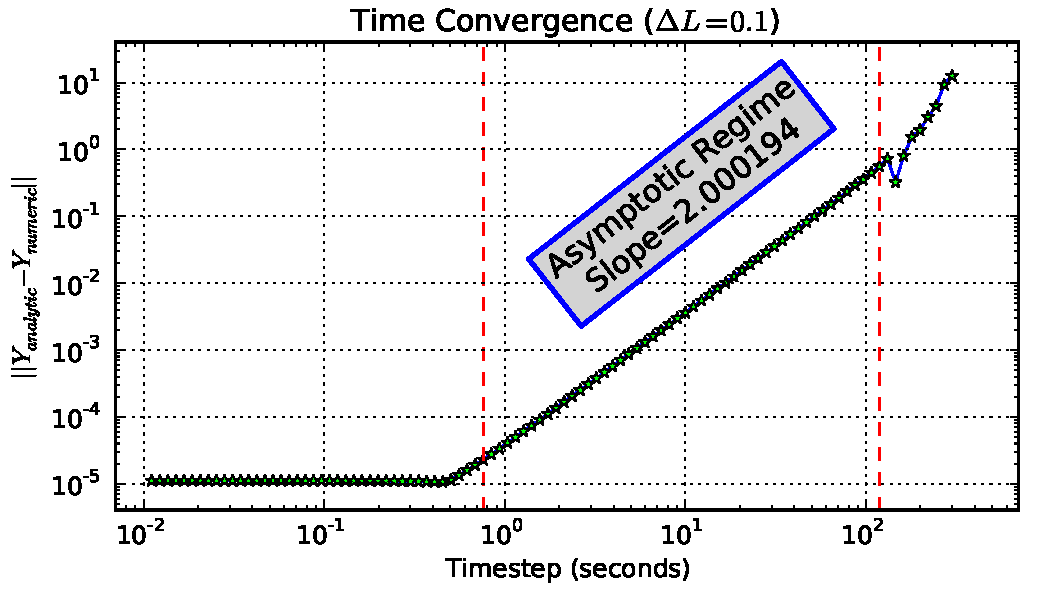
\includegraphics[width=10cm]{fig05_a.pdf}
  \end{center}
  \caption{Convergence as $\Delta t$ is refined while the spatial step, 
    $\Delta L$, is held constant.
    Each star represents the results from an individual simulation.
    The approximate location of the asymptotic regime is delimited by vertical
    red dashed lines.  The slope of the line indicates the order of convergence.
    From \citet{welling_rb}.}
  \label{f1}
\end{figure}

After some work, you note that for an initial condition of,
\begin{equation}
  U(x,0) = \sin(\pi x) + \sin(3 \pi x)
\end{equation}
the heat equation has an analytical solution, namely,
\begin{equation}
  U(x,t) = \sin(\pi x)e^{-\pi^2t}+\sin(3\pi x)e^{-9\pi^2t}
\end{equation}
With this information, it seems quite possible to verify that Ace's code works
(or not).

For this question, you must do the following:
\begin{enumerate}
  \item Create a main program unit that executes Ace's code using the
    initial conditions listed above.  Create a Makefile to compile your code.
  \item Fix Ace's code so that the missing module and associated subroutines
    are either replaced or are no longer needed, but the result is written 
    to file.
  \item Verify that the model converges correctly in both time and space.
    The Crank-Nicholson method is second order in both.
  \item Create a short write-up showing the code's convergence (or lack thereof).
\end{enumerate}

\bibliographystyle{plainnat}
\bibliography{dtw_bib}

\end{document}
